\chapter{Marco Teórico}\phantom{\cite{beetz09ijcss}}

Este capítulo va a poner en contexto al lector con respecto a conceptos básicos de criptografía para posteriormente explicar los algoritmos que van a ser implementados en el FPGA.\footnote{Según el ISO 7498-2 los términos correctos para encriptar y desencriptar son cifrar y descifrar respectivamente.}

\subsection{Conceptos Básicos}
Según la Real Academia Española \cite{} la criptografía se define como 
\newline
\newline
\emph{Arte de escribir con clave secreta o de un modo enigmático.}
\newline
\newline
El mensaje que se desea transmitir es usualmente llamado \textit{texto plano} o simplemente \textit{mensaje}. Este mensaje pasa por un proceso donde se disfraza el texto plano en un \textit{texto cifrado}, el proceso es llamado \textit{cifrado}. El proceso inverso donde se toma un texto cifrado en un texto plano se denomina \textit{descifrado}. 

El texto plano o mensaje se denota usualmente por la letra M o P, el texto cifrado se denota usualmente por la letra C, la función o algoritmo que cifra se denota por E y la que descrifa se denota por D. Se muestra en las Ecuaciones \ref{eqCifrado} y \ref{eqDescifrado} las relaciones entre estas notaciones. Note como al aplicarle la función de cifrado al texto plano se obtiene el texto cifrado y como al aplicarle la función de descifrado al texto cifrado se obtiene el texto plano. Finalmente se debe cumplir la identidad que describe la Ecuación \ref{eqCifraDescifra}. \cite{}
\begin{equation} \label{eqCifrado}
E(M) = C
\end{equation}
\begin{equation} \label{eqDescifrado}
D(C) = M
\end{equation}
\begin{equation} \label{eqCifraDescifra}
D(E(M)) = M
\end{equation}


\subsection{Sistema criptográfico \textit{criptosistema}}
Cuando la seguridad del algoritmo se basa en como procede el algoritmo, se denomina \textit{algoritmo restringido}. Este tipo de algoritmos son poco utilizados en la actualidad debido al gran problema que presentan. Tomemos de ejemplo que un grupo de usuarios decide utilizar un algoritmo de cifrado restringido para sus comunicaciones, se tendrá una comunicación segura hasta que alguno de los miembros decida salirse del grupo, ya que el usuario al no pertenecer más al grupo, no le importa mantener en secreto el algoritmo y puede distribuirlo para que terceros intercepen las comunicaciones de ese grupo. Así cada vez que un miembro deja el grupo, el grupo debe proceder a cambiarse a todo un nuevo algoritmo lo cual puede tornarse una labor complicada.

En cambio la criptografía moderna agrega el concepto de \textit{llave} donde se tiene un algoritmo el cual toma como parámetro de entrada una llave y el texto plano o texto cifrado y cifra o descifra el mismo, haciendo uso de la llave para su correcto desempeño. Así volviendo al ejemplo anterior, el grupo solamente necesitaría cambiar de llave cuando un miembro se va, facilitando el uso del cifrado y manteniendo las comunicaciones secretas.







En la actualidad se trabaja la criptografía sobre computadoras, es decir, cifrando y descrifrando bits, los cuales pueden tener diferentes significados, ya sea una imagen, un texto, un programa, etc. Esto significa que en la actualidad no se trabaja sobre caracteres del alfabeto o símbolos, sino más bien sobre 1's y 0's. Esto toma relevancia ya que al tener solo dos símbolos para cifrar, los algoritmos se vuelven más complejos por la falta de alternativas para sustituir un símbolo por otro.



\begin{figure}
	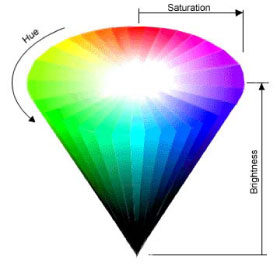
\includegraphics[width=0.4\linewidth]{images/hsb}
	\caption{Espacio de color HSI} \label{fig:hsb}
\end{figure}
\begin{figure}
	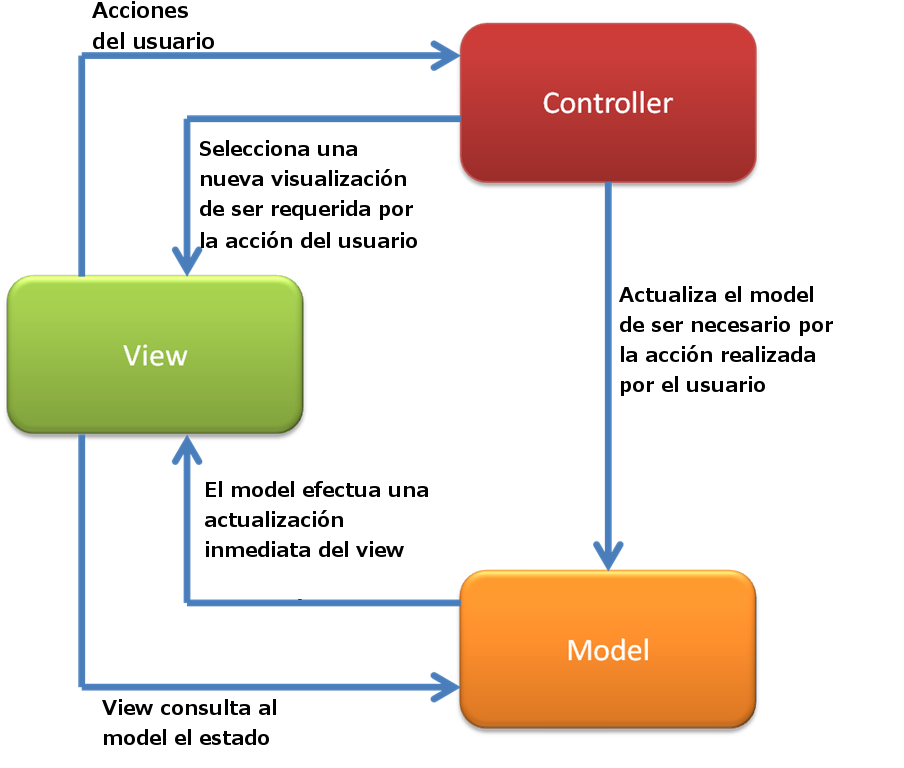
\includegraphics[width=1\linewidth]{images/mvcbase}
	\caption{Patrón de diseño MVC} \label{fig:mvc}
\end{figure}

